%imports
%=============================================================================================
\documentclass[a4paper,12pt]{article}
\usepackage[spanish, english]{babel}
\usepackage[utf8]{inputenc}
\usepackage{booktabs}
\usepackage{fontawesome}
\usepackage{graphicx}
\graphicspath{ {Graficos/} }
\usepackage{gensymb}
\usepackage{natbib}
\usepackage{caption}
\usepackage{pdfpages}
\usepackage[export]{adjustbox}
\usepackage{subfig}
\usepackage{a4wide}
\usepackage[colorlinks=true,linkcolor=black,urlcolor=blue,bookmarksopen=true]{hyperref}
%\usepackage{bookmark}
\usepackage{fancyhdr}
\usepackage[spanish]{babel}
\usepackage[utf8]{inputenc}
\usepackage[T1]{fontenc}
\usepackage{graphicx}
\usepackage{float}
\usepackage{fancyvrb}
\renewcommand*\ttdefault{txtt}
\usepackage[T1]{fontenc}
\usepackage{listings}
\usepackage{amssymb}
\usepackage{setspace}
\usepackage{helvet}
\usepackage{lmodern}
\usepackage{titlesec}
\usepackage{amsmath}

%para el titulo de la tabla de contenidos
%=============================================================================================
\addto\captionsenglish{
  \renewcommand{\contentsname}
    {Indice}
}
%=============================================================================================



%comienzo de documento
%=============================================================================================
\begin{document}
\title{
    \includegraphics[width=10cm]{"Logo FIUBA".jpg}\newline
    Teoría de Algoritmos I 75.29\\
    Trabajo Práctico N\textsuperscript{\underline{o}} 1\
}
\author{Grupo Rosita Forever}
\date{}
\setlength{\parindent}{0pt}

\pagenumbering{gobble}
\maketitle

\begin{table}[h!]
    \centering
	\begin{tabular}{ccc}
	    \toprule
		Apellido y Nombre & Padrón & Correo electrónico	\\
		\midrule
		Jamilis, Netanel David   & 99093 & njamilis@fi.uba.ar\\
		Del Torto, Agustín       & 98867 & adeltorto@fi.uba.ar\\
		Daverede, Agustín        & 98540 & agusdaverede@yahoo.com.ar \\
		Betz, Joaquín            & 104348 & \\
		\bottomrule
	  \end{tabular}
\end{table}
	
\verb Github: \faGithub \quad \faGithubSign \par
\extrainfo{
\url{{https://github.com/netaneldj/7529-TDA/TP1}} \newline}
\newpage
\pagenumbering{arabic}
\tableofcontents
\newpage

%secciones
%=============================================================================================
\section{Introducción}

\subsection{Objetivos}
Los objetivos del presente trabajo son los siguientes:
\begin{itemize}
\item Aplicar los conceptos aprendidos en clase en un problema Greedy
\item Aplicar los conceptos aprendidos en clase en un problema de División y Conquista
\item Preparar un informe técnico
\end{itemize}

En las siguientes secciones se vera plasmado el cumplimiento de los objetivos.\newline

\subsection{Resumen}
El presente trabajo se centrará en la presentación y consecuente resolución de los problemas planteados.\newline 
En primer lugar, se tratará el problema de ausentismo, perteneciente a la familia de problemas Greedy. Se analizará su solución y se planteará explicando el algoritmo empleado paso a paso.
Luego, se repetirá el mismo análisis para el problema de una nueva regulación industrial, donde se aplicará la estrategia de división y conquista.

En último lugar, se analizaran los resultados obtenidos, donde se tendrán en cuenta los conocimientos adquiridos en el desarrollo del trabajo y la bibliografía consultada para la realización del presente informe.

\newpage

 \section{Manifestaciones seguras}

En una decisión temeraria una ciudad decidió autorizar un conjunto de n manifestaciones el mismo día y horas. Cada manifestación comienza en un punto de reunión y tiene un destino final. Para evitar enfrentamientos y confusiones desean que cada ruta sea aislada de las otras. Contamos con el mapa de la ciudad que incluye todos los caminos e intersecciones por lo que pueden ir las marchas. Nos piden que elaboremos un algoritmo que retorne los caminos a seguir para cada manifestación de modo que no haya riesgo de un cruce (si es posible).\newline
Debemos demostrar que es un problema NP-Completo.
%=============================================

\subsection{Solución}
El problema que precede se puede modelar con un grafo en donde los nodos son las intersecciones de las calles y las aristas son las calles de la ciudad. En un principio todas las calles están disponibles para efectuar las manifestaciones siempre y cuando no se superpongan las manifestaciones.
%=============================================

\subsection{Demostración NP-Completo}
Para demostrar que es $\mathsf{NP-Completo}$ debemos demostrar que nuestro problema pertenece a $\mathsf{NP}$ y a $\mathsf{NP-Hard}$ simultáneamente.

\subsubsection{Demostración NP}
Para demostrar que el problema es $\mathsf{NP}$ debemos poder corroborar la solución propuesta en tiempo polinomial. Usando la analogía de la cerradura y la llave, esto sería equivalente a dada la llave probar que esta abre la cerradura en "tiempo polinomial". \newline

A continuación se propone un algoritmo que verifica la solución propuesta en tiempo polinomial:

\begin{verbatim}
Llamar L a la lista de manifestaciones(representadas por tuplas de nodos)

Funcion esManifestacionValida(L):
    Llamar visitados a la lista que contendrá a los nodos visitados
    
    visitados es lista vacia
    Para cada manifestacion en manifestaciones:
        Para cada esquina en manifestacion:
            Si esquina en visitados:
                Devolver falso
            Sino:
                visitados agregar esquina
    Devolver verdadero
\end{verbatim}

Se puede apreciar que la complejidad es de $\mathcal{O}(km)$ siendo $k$ la cantidad de manifestaciones y $m$ la cantidad máxima de esquinas atravesadas por una manifestación.

\subsubsection{Demostración NP-Hard}
Para demostrar que el problema es $\mathsf{NP-Hard}$, consideremos una instancia del problema conocido como conjunto independiente que consiste en un grafo $G=(V, E)$ con $|V|=n$ y un valor entero $k$.

\begin{figure}[H]
\centering
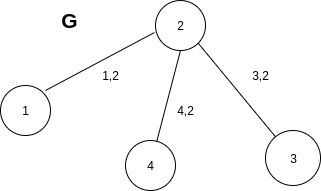
\includegraphics[width=0.9\textwidth]{Informe/Imagenes/Parte1/grafico 1.png}
\caption{\label{fig:class01}Instancia conjunto independiente}
\end{figure}

Sea el grafo $M = (V', E')$ donde $V' = V \cup \{ x_{u,v} \, : \, (u,v) \in E \}$ y $E' = V' \times (V'-1)$.

\begin{figure}[H]
\centering
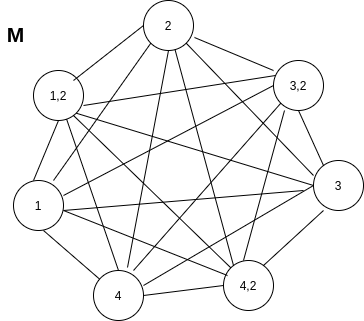
\includegraphics[width=0.9\textwidth]{Informe/Imagenes/Parte1/grafico 2.png}
\caption{\label{fig:class01}Grafo manifestaciones}
\end{figure}

Para cada $u \in V$ siendo $v_1, v_2, \dots, v_m$ los vecinos de $u$ en $G$ y definamos la ruta $P_u = \langle u, x_{u,v_1}, x_{u,v_2}, \dots, x_{u,v_m} \rangle⟩$ en $M$. Siendo $\mathcal{P} = \{P_u \, : \, u \in V\}$.\newline

Hay un conjunto independiente de tamaño como máximo $k$ en $G$, si y solo si hay un subconjunto $\mathcal{P}'$ con $|\mathcal{P}'| \le k$ tal que los caminos en $\mathcal{P}'$ son vértices disjuntos. \newline
Para visualizarlo, construimos los siguientes Paths en M: 

\begin{figure}[H]
\centering
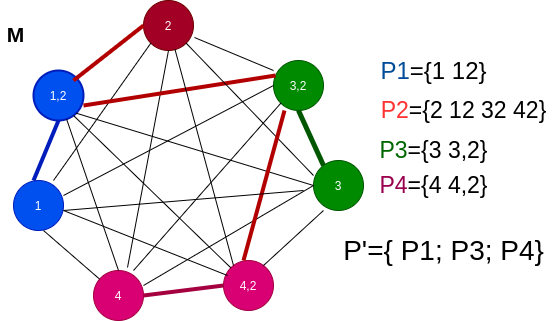
\includegraphics[width=0.9\textwidth]{Informe/Imagenes/Parte1/grafico 3.png}
\caption{\label{fig:class01}Rutas}
\end{figure}

Ahora queda formado un $\mathcal{P}'$ =  \{ P1; P3; P4 \} con $|\mathcal{P}'| = 3$ que representa en nuestro grafo G:

\begin{figure}[H]
\centering
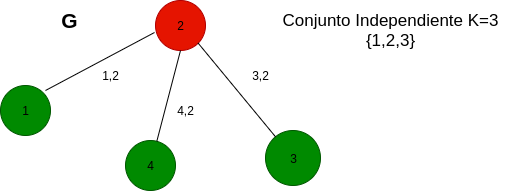
\includegraphics[width=0.9\textwidth]{Informe/Imagenes/Parte1/grafico 4.png}
\caption{\label{fig:class01}Nodos Independientes}
\end{figure}

Más precisamente, si $S$ es un conjunto independiente de $G$, entonces $\{ P_u \, : \, u \in S \}$ es una colección de caminos separados de vértices $M$ y, si $\mathcal{P}'$ es una colección de caminos separados de vértices en $M$, entonces $\{u \, : \, P_u \in \mathcal{P}' \}$ es un conjunto independiente de $G$.

\begin{figure}[H]
\centering
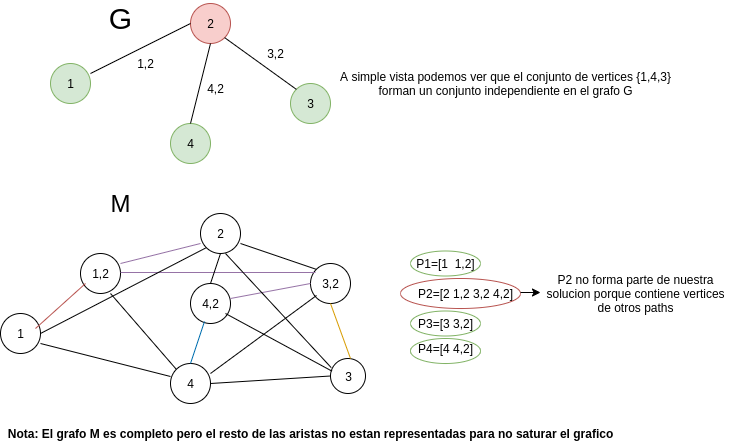
\includegraphics[width=1.148\textwidth]{Informe/Imagenes/Parte1/grafico 5.png}
\caption{\label{fig:class01} Vista General}
\end{figure}
%=============================================



\newpage

\section{División de Bienes}

Una de las parejas más ricas del mundo está pasando por un proceso de divorcio. Entre sus bienes cuentan con propiedades, autos, motos, estampillas raras y otros coleccionables. Como no se ponen de acuerdo en la manera de dividirlos, el juez ha dictaminado que un tasador ponga valor a cada bien y luego se haga una partición por valores iguales. El juez nos pide que elaboremos un algoritmo que en forma eficiente haga este trabajo.<<\newline
%============================================

\subsection{Solución}
El problema que precede se puede pensar como una representación de un conjunto

$C=\{w_{1}, w_{2}, ..., w_{n}\}$ donde cada $w_{i}$ está asociado al precio de cada bien. Luego, se desea determinar si existe un subconjunto de C tal que:

\begin{equation}
    W=\sum w_{i}
\end{equation}

Donde $w_{i}$ representa el precio de cada bien.

Utilizando conceptos de programación dinámica es posible llegar a una solución. No obstante, dicha solución estaría caracterizada por ser $O(W\cdot n)$, donde n es la cantidad de bienes y W es el valor de la ecuación (1) al que se desea llegar. Esto puede llegar a ser de orden casi exponencial si considera un W muy grande, y se tiene en cuenta la cantidad de bits empleados para representarlo y su crecimiento.

Sin embargo, como se describirá en el siguiente apartado, el problema es NP-Completo, de manera que no es posible hallar una solución que no sea exponencial. Al menos así ha sido descripto hasta ahora.

\subsection{Demostración NP-C}
%=============================================
Para poder demostrar que el problema es NP-Completo, se decidió proceder realizando la demostración a partir de dos hipótesis:
\begin{itemize}
    \item El problema es NP
    \item El problema es NP-Hard
\end{itemize}

Si ambas se cumplen, podemos afirmar que el problema es NP-Completo.

En primer lugar, se debe demostrar que es NP. Utilizando la notación previa, se puede decir que el subconjunto C puede tener tantos elementos como el conjunto original. Para poder hallar a W es preciso realizar las sumas asociadas a las iteraciones de los diferentes $w_{i}$. Esto se puede resolver en tiempo polinomial, luego el problema es NP.

Ahora se debe probar que el problema es NP-Hard. 

Para eso se va a demostrar:

\begin{equation}
    3DM \leq_{p} SUBSET-SUM
\end{equation}

La demostración se sustenta en que es conocido que el problema 3 dimensional matching es NP-C.

Para proceder a demostrar que el problema SUBSET SUM se puede reducir a 3DM se planteará que el conjunto C\subseteq X,Y,Z, siendo estos conjuntos ordenados disjuntos de tamaño n cada uno. Se desea determinar si existe el conjunto C.

Luego, se procede a representar a una tripla $t={x_{i}, y_{i}, z_{i}}$ como una serie de bits de tamaño 3n. A los efectos de resolver el problema se plantea que el conjunto C se puede representar como se demuestra a continuación:

\begin{figure}[H]
\centering
\includegraphics[width=0.7\textwidth]{Informe/Imagenes/Parte2/imagen1.png}
\caption{\label{fig:class01}Representación de tripla}
\end{figure}

No obstante, esta representación trae aparejado un posible problema de overflow. Esto se puede observar en la siguiente representación:

\begin{figure}[H]
\centering
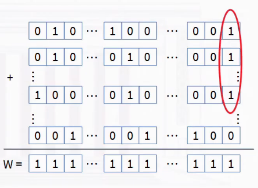
\includegraphics[width=0.5\textwidth]{Informe/Imagenes/Parte2/imagen2.png}
\caption{\label{fig:class01}Problema de overflow}
\end{figure}

Para evitar esta situación se debe elegir una representación en una base al menos un valor mayor de la cantidad de triplas, ya que esto imposibilita que se presente el overflow.

Al llegar a una representación del problema que se puede caracterizar por 3DM, podemos afirmar que el mismo representa a un problema similar a 3DM. 

Por lo tanto, como 3DM es NP-C, se probó la ecuación (2) y también que el problema es NP, se puede afirmar que se trata de un problema NP-C.
\newpage

\section{Un poco de teoría}
%=============================================
\subsection{Definiciones}
Defina y explique (si es necesario con ejemplos) qué significa que un problema sea P, NP, NP-Completo y NP-Hard
%=============================================

\subsection{Problema}
Tenemos un problema A, un problema B y una caja negra NA y NB que resuelven el problema A y B respectivamente. Sabiendo que B es NP
%=============================================
\subsubsection{I}
Qué podemos decir de A si utilizamos NA para resolver el problema B (asumimos que la reducción realizada para adaptar el problema B al problema A es polinomial)
%=============================================
\subsubsection{II}
Qué podemos decir de A si utilizamos NB para resolver el problema A (asumimos que la reducción realizada para adaptar el problema A al problema B es polinomial)\newline

Decimos que A es igual o menos complejo que B.
%=============================================

\subsubsection{III}
Qué pasa con los puntos anteriores si no conocemos la complejidad de B, pero sabemos que A es P?

\begin{enumerate}
    \item Decimos que A es igual o más complejo que B y ambos se pueden resolver de forma polinómica.
    \item Decimos que B es igual o más complejo que A y no necesariamente B se resuelve de forma polinómica.
\end{enumerate}
%=============================================


\newpage

\section{Conclusión}
Habiendo culminado el trabajo podemos efectuar las siguientes conclusiones:
%=============================================
 \subsection{Manifestaciones seguras}    
\begin{itemize}
    \item El problema se simplifica al modelar la ciudad como un grafo.
    \item Cada vértice independiente en \emph{Independet set} equivale a un camino independiente en nuestro problema
\end{itemize}
%=============================================
 \subsection{División de Bienes}    
\begin{itemize}
    \item 
\end{itemize}
%=============================================
\subsection{Un poco de teoría}    
\begin{itemize}
    \item Un problema solo puede ser resuelto por otro igual o más complejo que el primero
\end{itemize}
%=============================================

\newpage

\section{Bibliografia y Referencias}
\begin{itemize}
    \item J. Kleinberg, E. Tardos, Algorithm Design
    \item T. Cormen, C. Leiserson, R. Rivest, C. Stein, Introduction to Algorithms
    \item  Dr. Andrew Harrington, "Comp 363: Algorithms - Spring 2019" - Universidad Loyola Chicago.
\end{itemize}
 %=============================================
\newpage

\section{Anexo Manifestaciones seguras}

En una decisión temeraria una ciudad decidió autorizar un conjunto de n manifestaciones el mismo día y horas. Cada manifestación comienza en un punto de reunión y tiene un destino final. Para evitar enfrentamientos y confusiones desean que cada ruta sea aislada de las otras. Contamos con el mapa de la ciudad que incluye todos los caminos e intersecciones por los que pueden ir las marchas. Nos piden que elaboremos un algoritmo que retorne los caminos a seguir para cada manifestación de modo que no haya riesgo de un cruce (si es posible).\newline
Debemos demostrar que es un problema NP-Completo.
%=============================================

\subsection{Solución}
El problema que precede se puede modelar con un grafo en donde los nodos son las intersecciones de las calles y las aristas son las calles de la ciudad. En un principio todas las calles están disponibles para efectuar las manifestaciones siempre y cuando no se superpongan las manifestaciones.
%=============================================

\subsection{Demostración NP-Completo}
Para demostrar que es $\mathsf{NP-Completo}$ debemos demostrar que nuestro problema pertenece a $\mathsf{NP}$ y a $\mathsf{NP-Hard}$ simultáneamente.

\subsubsection{Demostración NP}
Para demostrar que el problema es $\mathsf{NP}$ debemos poder corroborar la solución propuesta en tiempo polinomial. Usando la analogía de la cerradura y la llave, esto sería equivalente a dada la llave probar que esta abre la cerradura en "tiempo polinomial". \newline

A continuación se propone un algoritmo que verifica la solución propuesta en tiempo polinomial:

\begin{verbatim}
Llamar L a la lista de manifestaciones(representadas por tuplas ordenadas de nodos)

Funcion esManifestacionValida(L):
    Llamo C al grafo que representa a la ciudad
    Llamar visitados a la lista que contendrá a los nodos visitados
    
    visitados es lista vacia
    Para cada manifestacion en L:
        Para cada esquina en manifestacion:
            Llamo S a siguiente esquina
            Si esquina en visitados:
                Devolver falso
            Si existe S y no existe camino(esquina,S):
                Devolver falso
            Sino:
                visitados agregar esquina
    Devolver verdadero
\end{verbatim}

Se puede apreciar que la complejidad es de $\mathcal{O}(km)$ siendo $k$ la cantidad de manifestaciones y $m$ la cantidad máxima de esquinas atravesadas por una manifestación.

\subsubsection{Demostración NP-Hard}
Para demostrar que el problema es $\mathsf{NP-Hard}$, consideremos una instancia del problema 3-SAT compuesto por $m$ clausuras y $n$ variables:\newline

$E = (X_{1}+X_{2}+X_{3})*(\overline{X_{1}}+\overline{X_{2}}+\overline{X_{4}})*(\overline{X_{2}}+\overline{X_{3}}+X_{4})$\newline

Para crear el grafo en el que se resolverá el problema de las manifestaciones definimos para cada variable ($i$ de $1$ a $n$) y para cada clausura ($j$ de $1$ a $m$) dos vértices: $X_{ij}$ ($true$) y $\overline{X_{ij}}$ ($false$); creando así 6 vértices por clausura. A su vez definimos un par de vértices $I$ (inicio) y $F$ (fin) por cada clausura y por cada variable quedándonos así formados los pares $I_{jc}$, $F_{jc}$ (para los pares de las clausuras) y $I_{iv}$, $F_{iv}$ (para los pares de las variables).\newline

Por cada clausura conectaremos $I_{jc}$ a $X_{ij}$ si la variable $X_{ij}$ esta sin negar y por consiguiente a $\overline{X_{ij}}$ si la variable esta negada y luego conectaremos la variable $X_{ij}$ usada al $F_{jc}$ correspondiente.\newline

Por cada variable conectaremos $I_{iv}$ al vértice $X_{ij}$ cuya $j$ sea la clausura de menor índice en la que aparezca la variable $i$, después conectaremos dicho $X_{ij}$ al $X_{ij}$ cuya $j$ sea la segunda clausura de menor índice en el que aparezca la variable $i$, crearemos aristas hasta que ya no queden clausuras que utilicen la variable $i$ y procederemos a unir el ultimo $X_{ij}$ al $F_{iv}$. Realizaremos exactamente el mismo procedimiento con las variables $\overline{X_{ij}}$. \newline

De esta forma nos queda el siguiente grafo: \newline

\begin{figure}[H]
\centering
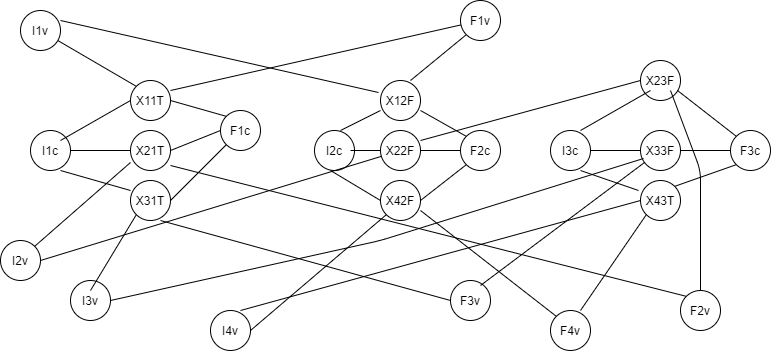
\includegraphics[width=0.9\textwidth]{Informe/Imagenes/Parte1/grafico 2-bis.png}
\caption{\label{fig:class01} Grafo manifestaciones}
\end{figure}

\underline{Nota:} No se muestran en el grafo los $X_{ij}$ que se encuentran aislados del resto para no sobrecargar al mismo y facilitar su comprensión.\newline

Por ultimo definiremos las manifestaciones. Existirá una manifestación por clausura, esta iniciara en el nodo $I_{jc}$ y finalizara en el $F_{jc}$ y otra manifestación por cada variable la cual iniciara en el nodo $I_{iv}$ y finalizara en el $F_{iv}$.\newline

Entonces en relación al problema de 3-SAT el camino que tomen las manifestaciones de las clausuras será la evaluación literal de $true$ de la variable y el camino que no usemos de las manifestaciones de las variables corresponderá a la asignación de $true$ a la variable. \newline

%=============================================



\newpage

\section{Anexo División de Bienes}

Una de las parejas más ricas del mundo está pasando por un proceso de divorcio. Entre sus bienes cuentan con propiedades, autos, motos, estampillas raras y otros coleccionables. Como no se ponen de acuerdo en la manera de dividirlos, el juez ha dictaminado que un tasador ponga valor a cada bien y luego se haga una partición por valores iguales. El juez nos pide que elaboremos un algoritmo que en forma eficiente haga este trabajo.\newline
%============================================

El pedido se puede plantear como un problema \textit{NUMBER-PARTITION}; dado un conjunto $C=\{w_{1}, w_{2}, ..., w_{n}\}$, donde cada $w_{i}$ está asociado al precio de cada bien, se desea determinar si existe un subconjunto W de C tal que la suma de sus elementos equivalga a la suma de los elementos restantes en C.

\begin{equation}
    \sum_{w\in W} w  = \sum_{w\in\overline{W}} w
\end{equation}

Para que un problema X sea NP-Completo, debe cumplirse que: \\
(1) $X$ sea NP\\
(2) cualquier problema NP-Completo $Y$ puede reducirse a $X$, en tiempo polinomial\\
(3) $X$ tenga una solución si y sólo si $Y$ tiene solución

\subsection{Demostración NP}

Corroborar que dos particiones de un conjunto sean solución de este problema es muy simple.  Sólo hay que verificar que la suma total de sus elementos sea equivalente. 
Por lo tanto, verificarlo es $\mathcal{O}(n)$, siendo n la cantidad de elementos del subconjunto más poblado. 
Entonces, al poder verificar la solución en tiempo polinomial, se puede asegurar que este problema es NP.

\subsection{Reducción del problema SUBSET-SUM}
Un conocido problema NP-Completo es el problema de la suma de los subconjuntos. 
Éste se puede describir como: Dado un conjunto de enteros $A$, ¿existe un subconjunto $S \subset A$, tal que la suma de sus elementos sea exactamente $k$?

En términos matemáticos:

\begin{gather*}
    A = \{w_{1}, w_{2}, ..., w_{n}\}, \sum_{w \in A} w_{i} = s \\
    \exists S \subset A  / \sum_{w \in S} w_{i} = k ?
\end{gather*}
Lo que se desea corroborar ahora es si \textit{SUBSET-SUM} $ \leq_{p} $ \textit{NUMBER-PARTITION}.
A tales efectos, se procederá a adaptar el problema \textit{SUBSET-SUM} para que sea resoluble a través de \textit{NUMBER-PARTITION}. 

Sea $s$ la suma de los miembros de $A$ y $A' = A \cup \{s-2k\}$ un conjunto definido, donde k es el valor objetivo previamente mencionado. Se aceptará que $A$ tiene solución si y sólo si \textit{NUMBER-PARTITION} acepta $A'$.

\begin{equation}
    A' = \{w_{1}, w_{2}, ..., w_{n}, s-2k\}, \sum_{w \in A'} = s + (s-2k) = 2s-2k
\end{equation}

Se desea probar que
$\{A,k\}$ $\in $ \textit{SUBSET-SUM} $\Leftrightarrow$ $\{A'\}$ $\in$ \textit{NUMBER-PARTITION}. Se hará esto en ambos sentidos.

\subsubsection{$\{A,k\}$ $\in $ \textit{SUBSET-SUM} $\Rightarrow$ $\{A'\}$ $\in$ \textit{NUMBER-PARTITION}}
 Si existe un conjunto de números en $A$ que sumen $k$, entonces el resto de los números sumarán $s-k$. 
\begin{gather*}
    S \subset A  / \sum_{w \in S} w = k \\
    \Rightarrow \sum_{w \in \overline{S}_{A}} w = \sum_{w \in A} w - \sum_{w \in S}w = s - k\\
\end{gather*}
Se llamará $\overline{S}$ al complemento de S en A. Entonces, es posible descomponer $A'$ de la siguiente forma (haciendo abuso de notación, pues $A$ y $A'$ son conjuntos casi idénticos).
    \begin{equation*}
    \begin{split}
        A' &= A \cup  \{s-2k\} \\
            &= \{\overline{S} \cup S\} \cup \{s-2k\} \\
            &= \overline{S}  \cup \{ S \cup \{s-2k\}\} \\
            &= B \cup \overline{B}_{A'}\\\              
    \end{split}
    \end{equation*}
Como $B \equiv \overline{S}$, la suma de sus elementos es "$s-k$". Luego, es posible calcular cuánto suma el conjunto de números restantes en A' (complemento de $B$ en $A'$).
    \begin{equation*}
    \begin{split}
    \sum_{w \in \overline{B}_{A'}} w & = \sum_{w \in A'} w - \sum_{w \in B} w \\
                            & =  2s-2k - (s-k) = s - k
    \end{split}
    \end{equation*}
    
Por lo tanto, existe una partición en dos de $A'$ ($B$ y $\overline{B}_{A'}$) tal que cada conjunto sume "$s-k$" (exactamente la mitad de la suma total de $A'$). 

\subsubsection{$\{A,k\}$ $\in $ \textit{SUBSET-SUM} $\Leftarrow$ $\{A'\}$ $\in$ \textit{NUMBER-PARTITION}} 
Si existe una partición en dos de $A'$ tal que cada una sume $s-k$ (la mitad de su suma), entonces una de ellas necesariamente contiene el número $s-2k$ que se agregó previamente. Al descartar del conjunto este valor, se obtiene un subconjunto de $A'$ cuya suma sea $k$.

\subsubsection{Corolario}
Un problema NP-Completo, como lo es el SUBSET-SUM, es reducible al problema del enunciado, NUMBER-PARTITION. Esta reducción es claramente en tiempo polinomial; para adaptar el conjunto "de entrada" sólo hay que incluir un valor (s-2k) para que pueda ser resuelto como una instancia de NUMBER-PARTITION. Además, para adaptar su salida sólo habría que identificar la partición con el valor que se agregó y descartarlo.\\
Teniendo todo esto en cuenta, se cumplen las 3 condiciones enunciadas y queda demostrado que NUMBER-PARTITION es NP-Completo porque, para poder resolverlo, se debe resolver el problema SUBSET-SUM, que es NP-completo.
\newpage

\section{Anexo Un poco de teoría}
%=============================================
\subsection{Definiciones}
\subsubsection{Problemas P y NP}
Un problema P es todo aquel problema de decisión que se puede resolver eficientemente (es decir, en tiempo polinomial), mientras que un problema NP es el que, contando con una posible solución del mismo, ésta se puede verificar eficientemente.\\

\subsection{NP-completo y NP-hard}
Si todo problema NP se puede reducir al problema A, A es un problema NP-hard. Y los NP-complete son aquellos problemas NP-hard que además son NP.\\

\subsection{Complejidad}
Si quisiéramos ordenar estos problemas de menor a mayor complejidad, en términos generales: 
\begin{itemize}
    \item P
    \item NP
    \item NP-Completo
    \item NP-Hard
\end{itemize}

\subsection{Ejemplos}
\begin{itemize}
    \item Problema P, NP: Camino más corto.
    \item Problema NP-completo: Problema de la mochila.
    \item Problema NP-hard: Problema de la parada.
\end{itemize}

%=============================================

\subsection{Problema}
Tenemos un problema A, un problema B y una caja negra NA y NB que resuelven el problema A y B respectivamente. Sabiendo que B es NP
%=============================================
\subsubsection{I}
Qué podemos decir de A si utilizamos NA para resolver el problema B (asumimos que la reducción realizada para adaptar el problema B al problema A es polinomial)\newline

Podemos decir que A es igual o menos complejo que B.
%=============================================
\subsubsection{II}
Qué podemos decir de A si utilizamos NB para resolver el problema A (asumimos que la reducción realizada para adaptar el problema A al problema B es polinomial)\newline
¿Por qué no podemos decir nada de A? ¿A quién le podemos pasar? ¿A qué clases puede (y no puede) pertenecer A? ¿Cómo es la relación de A con respecto a B?\newline

Ya que A se puede resolver con NB sabemos que no es un problema mas complejo que NP. Sin embargo A puede pertenecer a cualquier complejidad menor a NP porque el que lo podamos resolver como  resolveriamos un problema NP no significa que no exista un metodo mas simple y de menor complejidad algoritmica para llegar al mismo resultado. Lo que si podemos asegurar es que A es de igual o menor complejidad que B.

%=============================================

\subsubsection{III}
Qué pasa con los puntos anteriores si no conocemos la complejidad de B, pero sabemos que A es P?\newline
Si “no necesariamente B se resuelve de forma polinómica”, ¿a qué clases puede pertenecer?

\begin{enumerate}
    \item Decimos que A es igual o más complejo que B y ambos se pueden resolver de forma polinómica.
    \item Decimos que B es igual o más complejo que A y no necesariamente B se resuelve de forma polinómica. B podría pertenecer a NP (o mayor) y que utilicemos un algoritmo de mayor complejidad para resolver un problema P.
\end{enumerate}
%=============================================


\newpage

\end{document}
%=============================================================================================
